\section{Comparison with the Python results of report 2}
\label{sec:python}

Report~2 used two nose terms from the Python tool. They are compared here with Fluent at the same free
stream and reference area.
\begin{itemize}
\item \textbf{Wave drag}: Euler simulations (no viscosity, pointed tip) interpolated to $L/D = 3.117$.
Below $M = 1.1$ there were no Euler runs, so the tool uses an assumed ramp:
\begin{equation}
C_{D,w}(M) = C_{D,w}(1.1)\; s^2(3 - 2s), \qquad s = \frac{M - 0.8}{0.2}\ \text{clipped to } [0, 1].
\end{equation}
Compared with Fluent's pressure part.
\item \textbf{Friction}: turbulent flat plate on the nose alone, smooth wall:
\begin{equation}
C_f = \frac{0.455}{(\log_{10}\mathrm{Re}_L)^{2.58}} \times
\begin{cases} 1 - 0.1M^2, & M < 1,\\ (1 + 0.15M^2)^{-0.58}, & M > 1, \end{cases}
\qquad C_{D,f} = C_f\,\frac{S_{\rm wet}}{A_{\rm ref}}, \quad S_{\rm wet} = \SI{0.2243}{m^2}.
\end{equation}
Compared with Fluent's viscous part.
\end{itemize}

\begin{table}[H]
\centering
\caption{Nose drag of study~A: Python (report~2) and Fluent. Difference = Fluent / Python $-$ 1.}
\label{tab:python}
\small
\begin{tabular}{@{}lrrrrrr@{}}
\toprule
 & \multicolumn{3}{c}{pressure (wave) $C_D$} & \multicolumn{3}{c}{friction (viscous) $C_D$} \\
\cmidrule(lr){2-4}\cmidrule(l){5-7}
$M$ & Python & Fluent & difference & Python & Fluent & difference \\
\midrule
0.95 & 0.0768 & 0.0042 & $-94.5$\,\% & 0.0236 & 0.0248 & $+5.2$\,\% \\
1.2 & 0.0926 & 0.0948 & $+2.4$\,\% & 0.0225 & 0.0224 & $-0.5$\,\% \\
1.47 & 0.0941 & 0.0963 & $+2.4$\,\% & 0.0210 & 0.0207 & $-1.4$\,\% \\
\bottomrule
\end{tabular}

\end{table}

\begin{figure}[H]
\centering
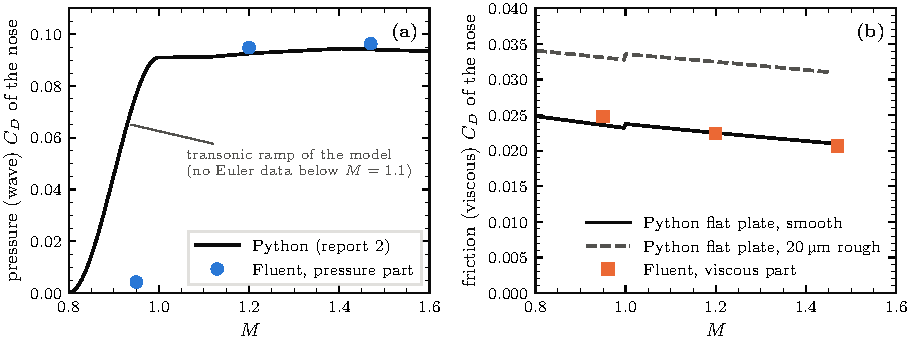
\includegraphics[width=\linewidth]{fig_python_compare}
\caption{(a) Wave drag of the Python model against Mach, and Fluent's pressure part. (b) Python
flat-plate friction of the nose along the boost of the report-2 trajectory (the Reynolds number changes
with $M$), for a smooth wall and for the \SI{20}{\micro m} roughness of the trajectory model, and
Fluent's viscous part. The small step at $M = 1$ is where the Python formula switches from its
subsonic to its supersonic compressibility correction.}
\label{fig:python}
\end{figure}

\paragraph{Supersonic: $+2.4\,\%$ at both Mach numbers.} Fluent has the real \SI{4.5}{mm} rounded tip and a
boundary layer that makes the nose act slightly fatter; both add a little pressure drag. With the
sensitivity of report~2 ($\approx\SI{7}{m}$ of apogee per per cent of wave drag), $+2.4\,\%$ costs about
\SI{17}{m}.

\paragraph{Friction: within $-1.4\,\%$ to $+5.2\,\%$.} The flat plate models the nose friction well. The
\SI{20}{\micro m} roughness of the trajectory model adds 40--47\,\% (dashed line), which these smooth-wall
runs do not check.

\paragraph{Transonic: Python is conservative.} At $M = 0.95$ the ramp gives 0.0768 ($s = 0.75$, so
84\,\% of the $M = 1.1$ value); Fluent gives 0.0042. The drag rise comes later and steeper than assumed,
so the drag of report~2 is too high between $M \approx 0.8$ and 1.0 and its apogee is on the safe side.
Placing the rise needs a Fluent run at $M = 1.0$--1.1 (Section~\ref{sec:conclusions}).
